\chapter{Evaluation}
In this chapter, we evaluate the prepared log files of our game to study the effectiveness and efficiency of the obfuscated queries. We have a look at some general aspects like the distribution of the obfuscated queries among players and their preferences regarding the categories and levels. Then we compare the average length of queries formulated by the participants with the length of the sensitive queries. We also investigate the overall success rate (target document retrieved) of players and the Mean Reciprocal Rank of the participants' queries in our document sample and ChatNoir. Finally, we categorize the obfuscated queries into five different types and compare their effectiveness to each other and to queries automatically obfuscated with the approach of Arampatzis et al.~\cite{arampatzis}.\par
We recruited users for our query obfuscation game from an information retrieval course and dedicated mailing lists at our universities (Bauhaus Universit{\"a}t Weimar, Martin-Luther-Universit{\"a}t Halle-Wittenberg). The information retrieval course was held at the Martin-Luther-Universit{\"a}t Halle-Wittenberg ($\approx$ 20 students). As a result, we were able to acquire 72 players which submitted a total of 1.534 obfuscated queries, 1.476 of those unique. 38 of the players completed a demographic survey which revealed that 13 were female, 25 male and their age ranged from 19 to 64 years.\par
There is great variance among the players regarding the number of their obfuscated queries. About 42\% of the players only submitted one to five queries and about 18\% submitted six to ten. This means that most players ($\approx$ 60\%) played one or two game rounds. As we can see in Figure~\ref{fig:distribution:num:queries}, the number of participants who submitted more than ten queries declines with increasing query quantity. However, we had one very engaged player who alone submitted a total of 499 obfuscated queries.  
\begin{figure}[h]
    \centering
    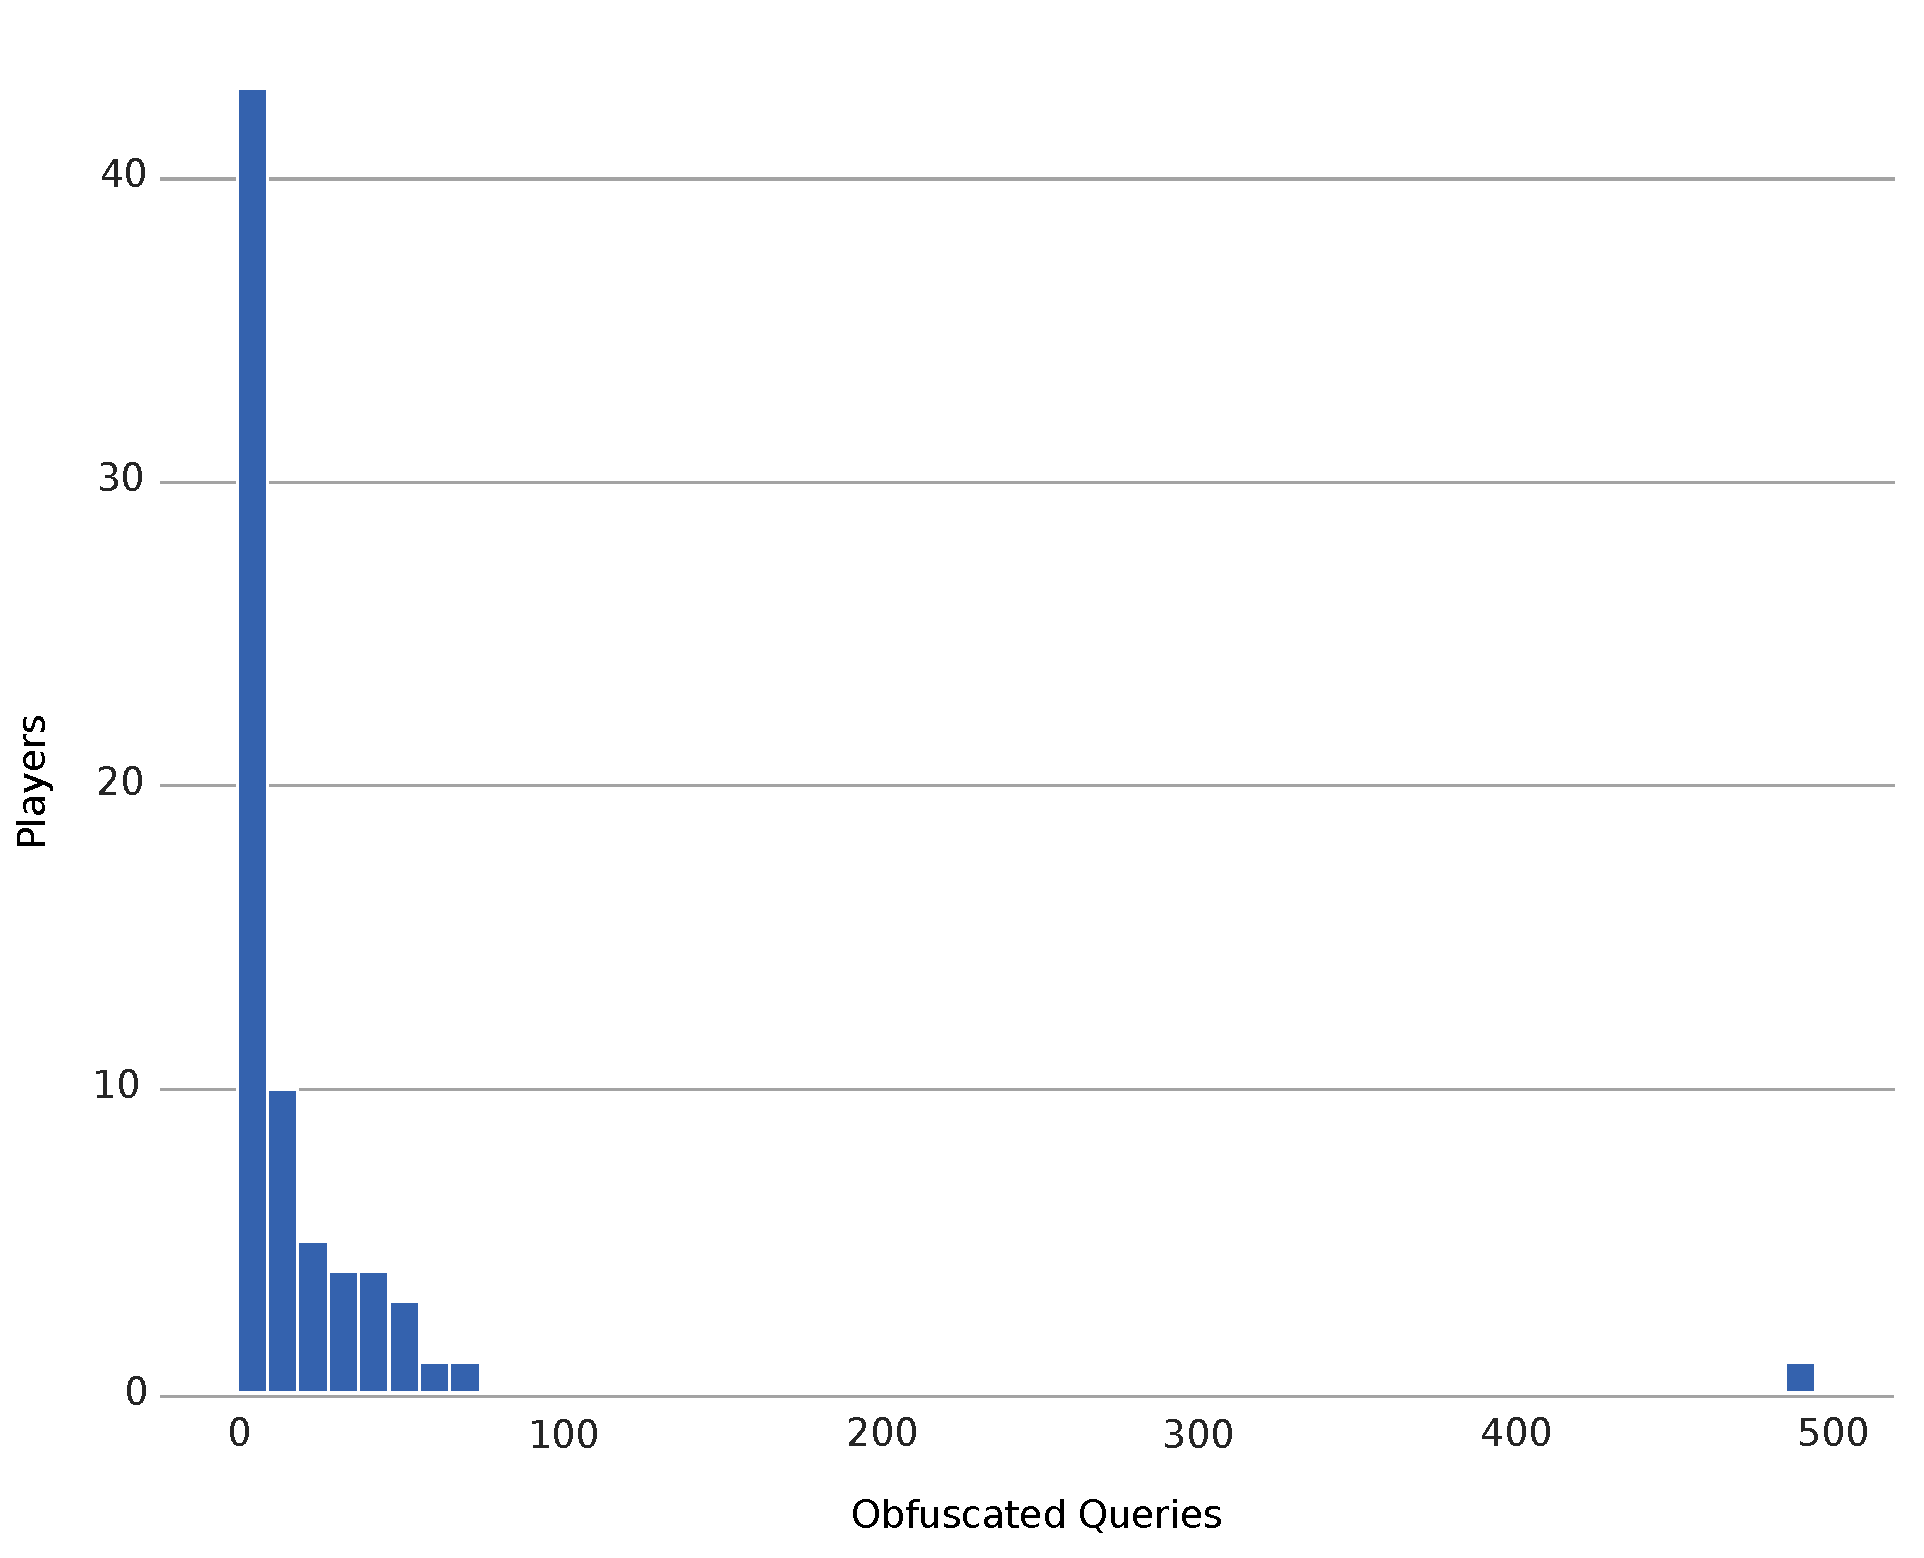
\includegraphics[width=0.7\textwidth]{graphics/evaluation/distribution_num_submitted_queries.pdf}
    \caption{Distribution of the amount of obfuscated queries among the players.}
    \label{fig:distribution:num:queries}
\end{figure}
The collected queries spread over the two levels we implemented, Squid and Chameleon, even though most players preferred the level Squid. Only 13\% of the collected queries were made in the level Chameleon, and only 18 participants decided to play this level. This can be explained, among other things, by the fact that the second level Chameleon is only unlocked after a participant successfully obfuscated five queries. Successful in this context means that the target document was retrieved. But since numerous players submitted very few queries, many did not even reach the second level.
However, it is noticeable that approximately 79\% of the queries in the level Chameleon were created without the usage of one of the provided auxiliary keywords (see Figure~\ref{fig:chameleon:intention}). This shows that the intention behind the level, to encourage the players to be more creative, was successful, even if the level itself was not very popular.\par
\begin{figure}[h]
    \centering
    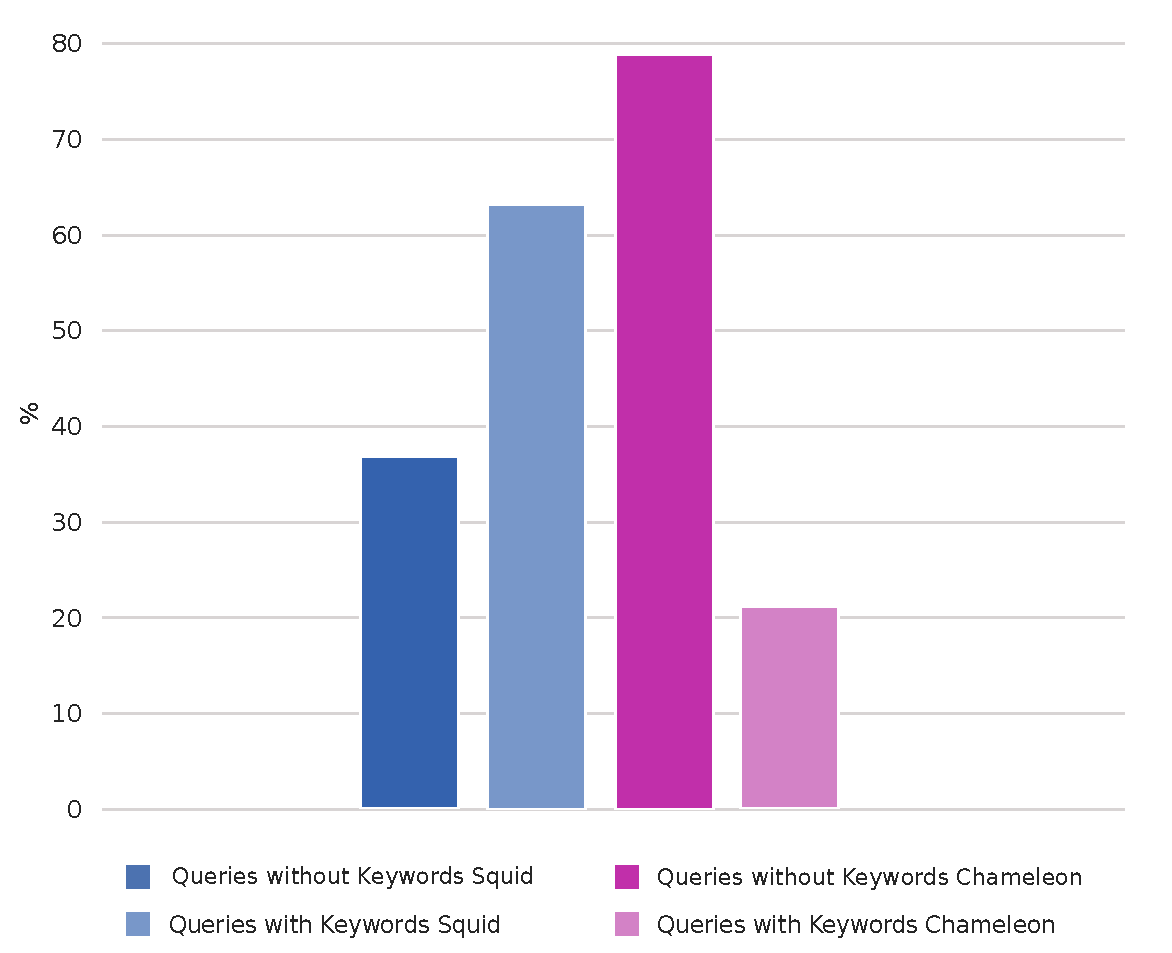
\includegraphics[width=0.6\textwidth]{graphics/evaluation/query_used_keyword_test_success_chameleon_purpose.pdf}
    \caption{The distribution of queries that were created with the help of a provided keyword.}
    \label{fig:chameleon:intention}
\end{figure}
Apart from the levels, there were also differences in the popularity of the individual categories. This can be seen from the number of obfuscated queries in each category (see Figure~\ref{fig:distribution:level:queries}). The category Knowledge was by far the most favored. If we look at the level Squid, almost all other categories are equally popular, except for Law. In the level Chameleon, the differences between the categories are not completely the same as in the other level but even here the category Knowledge was the most popular and law the most disliked. This is an interesting distribution since it shows that the number of sensitive queries in one category is not related to the number of obfuscated queries in this category. Because if this were the case then most queries would have been obfuscated in the categories Health and Personal. But these are on par with a category like politics which does not even consist of half as many queries.\par
\begin{figure}[h]
    \centering
    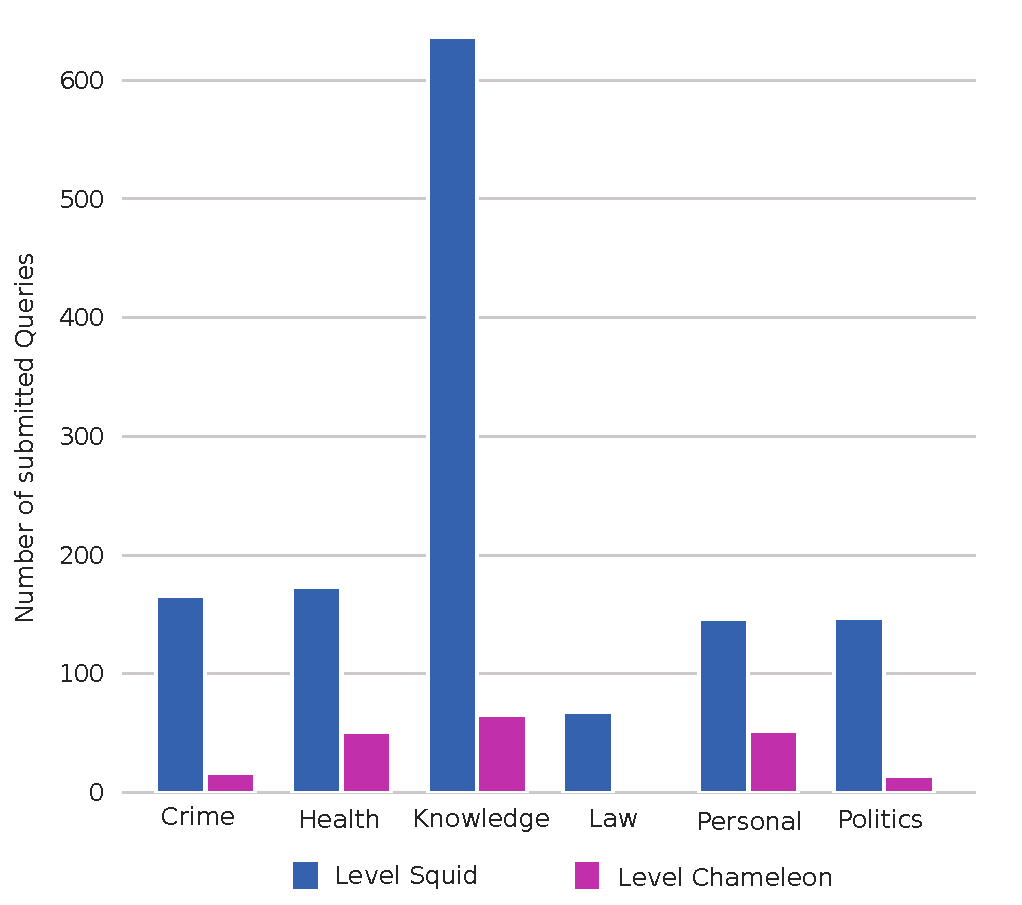
\includegraphics[width=0.6\textwidth]{graphics/evaluation/queries_per_category.pdf}
    \caption{This graph shows the number of obfuscated queries that were submitted in each category and level.}
    \label{fig:distribution:level:queries}
\end{figure}
Although there are differences in the popularity of the different queries, we can see that in each category the average length (in terms) of the created queries was longer than the original sensitive queries (see Figure~\ref{fig:distribution:length:categories}). 
\begin{figure}[h]
    \begin{minipage}[b][][b]{0.47\textwidth}
        \centering
        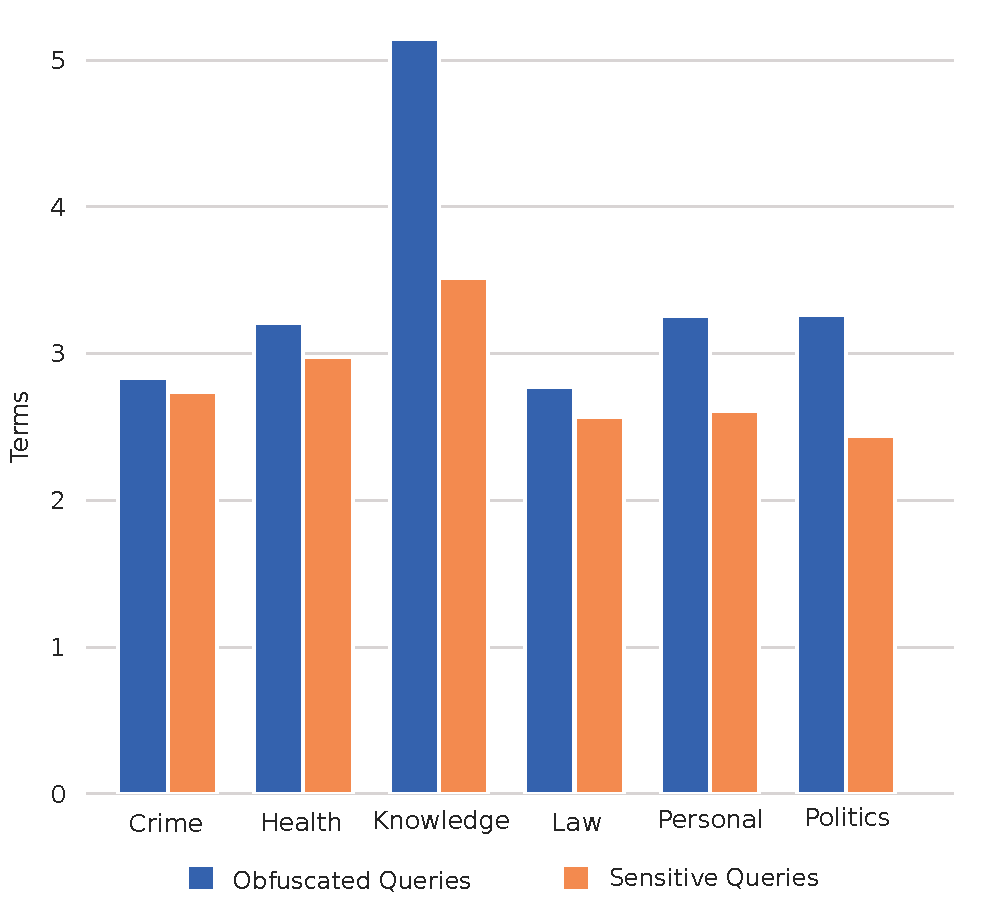
\includegraphics[width=1.0\textwidth]{graphics/evaluation/queries_length_comparison_original_categories.pdf}
                \caption{Comparison of the average length of the obfuscated queries with the sensitive queries in each category.}
    \label{fig:distribution:length:categories}
    \end{minipage}
    \hfill
    \begin{minipage}[b][][b]{0.47\textwidth}
        \centering
        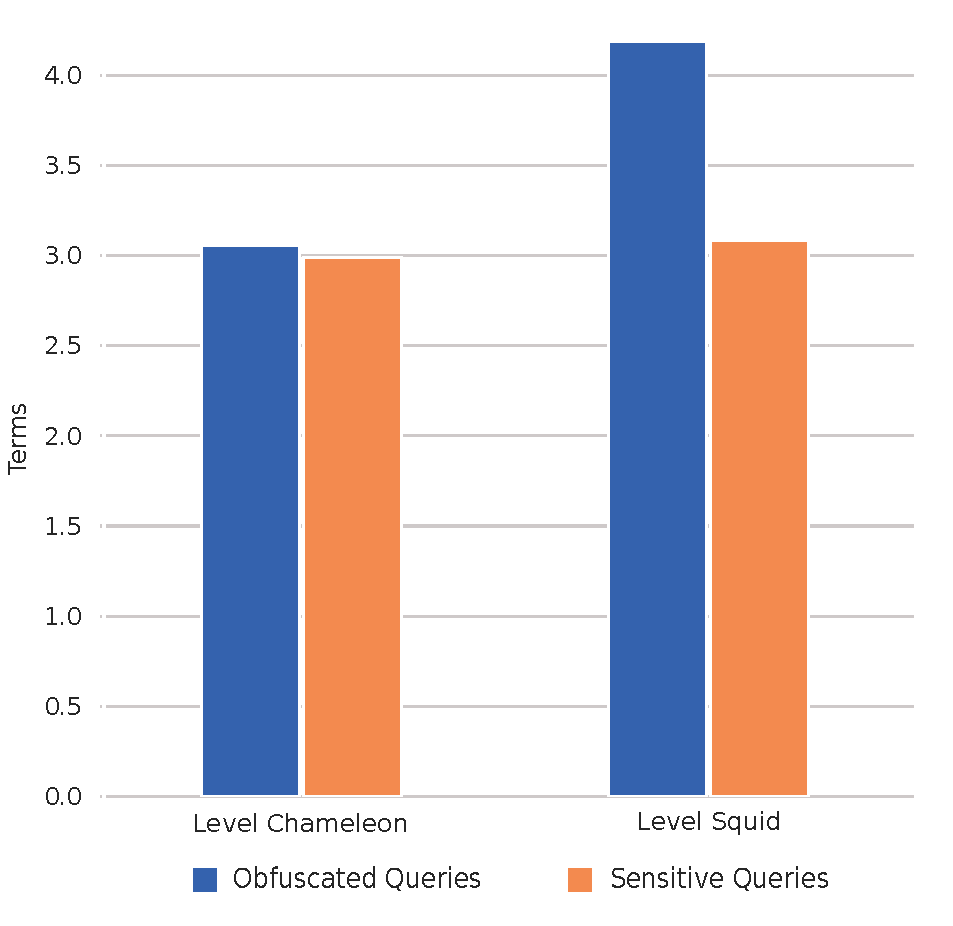
\includegraphics[width=1.0\textwidth]{graphics/evaluation/queries_length_comparison_original.pdf}
                    \caption{Comparison of the average length of the obfuscated queries with the sensitive queries in the two levels.}
        \label{fig:distribution:length:level}
    \end{minipage}
\end{figure}
The most significant difference in length can be seen in the category Knowledge. Also mentionable is the fact that the length difference between the sensitive and obfuscated queries is bigger in the level Squid than in the level Chameleon (see Figure~\ref{fig:distribution:length:level}). 
This discrepancy could be explained by the different number of submitted queries and players between the two levels. More distinct players and queries hold more potential for different approaches when it comes to obfuscating queries. Additionally, the level Squid contains the longest obfuscated query with 55 terms which also increases the average length for this level.
In general, the average length of the submitted queries is 4.04 which is in the normal range of 2-4 terms~\cite{arampatzisLength}. Figure~\ref{fig:distribution:length} shows that most submitted queries have a length of 2-4 terms but longer queries also occur. However, the length of the obfuscated queries is above the average length of the sensitive queries, which is 3.07 terms. Other sources also indicate that normal queries are on average 3.31~\cite{fu-finder} or 3.5~\cite{pictureSearch} terms long. Even though these sources show a slight deviation among themselves, their values are still lower than our value for the average length of the obfuscated queries.\par


\begin{figure}[b]
    \vspace*{-.5cm}
    \begin{minipage}[b][][b]{0.45\textwidth}
    \centering
    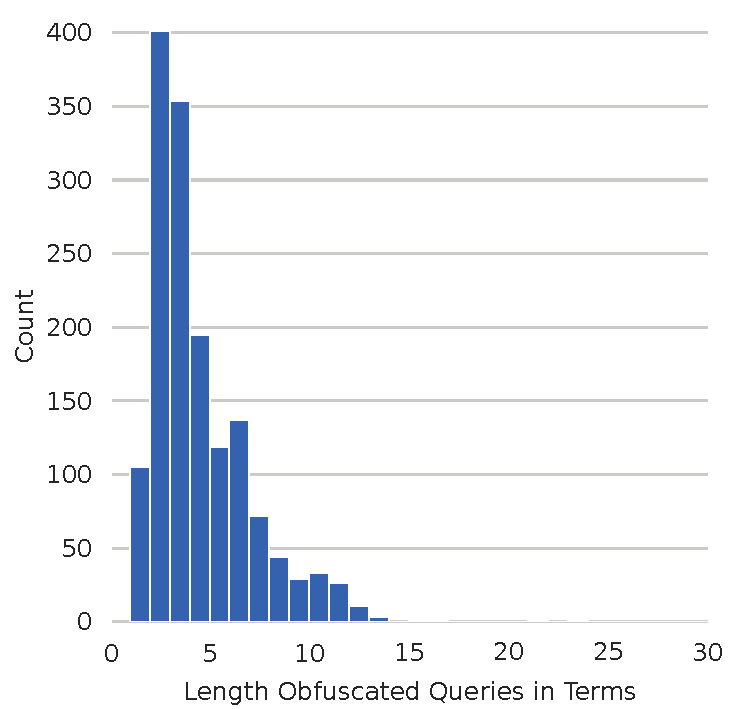
\includegraphics[width=1.0\textwidth]{graphics/evaluation/distribution_length_submitted_queries.pdf}
    \caption{The distribution of the length of the obfuscated queries.}
    \label{fig:distribution:length}
    \end{minipage}
    \hfill
    \begin{minipage}[b][][b]{0.45\textwidth}
    \centering
    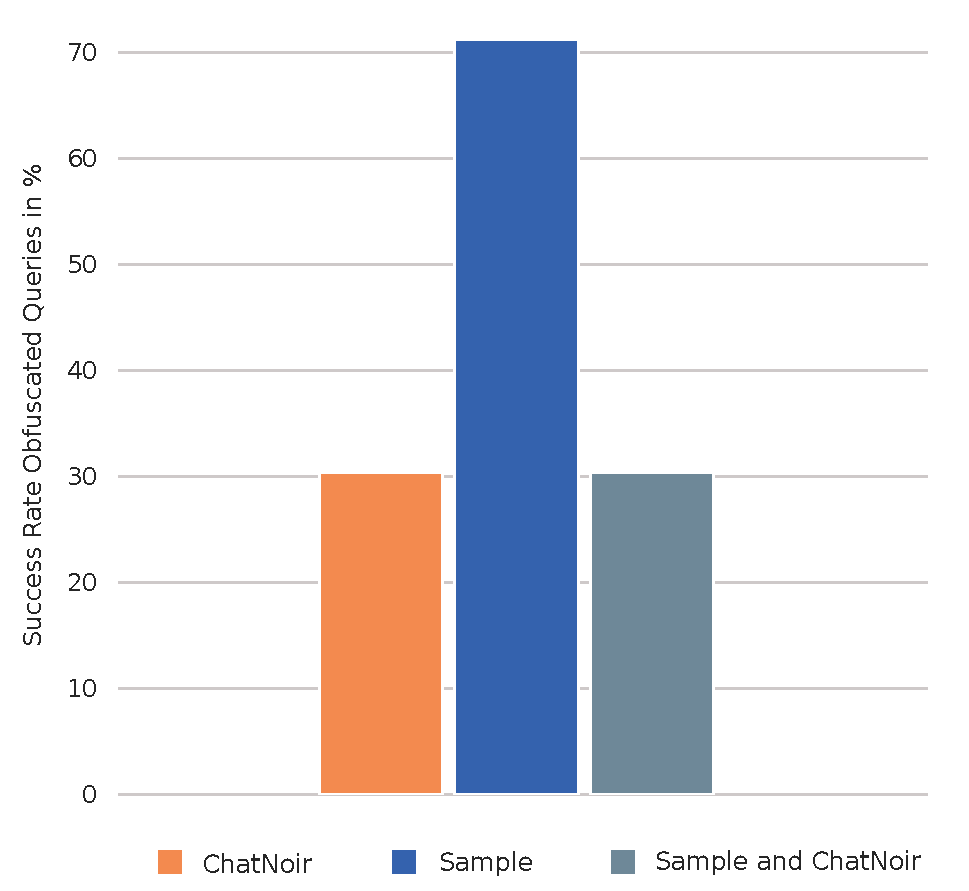
\includegraphics[width=1.0\textwidth]{graphics/evaluation/successrate_users.pdf}
    \caption{Success rate of queries in ChatNoir and our document sample.}
    \label{fig:successrate:users}
    \end{minipage}
\end{figure}
Another aspect that we investigated is the overall success rate of players. The success rate is defined as the percentage of queries that successfully retrieved the target document. As Figure~\ref{fig:successrate:users} shows, the success rate in the document sample (Index) is more than twice as high as the success rate in the ClueWeb12 (70\% compared to 30\%). We can also see that if the target document gets retrieved in ChatNoir then it also gets retrieved in our sample. Another thing we can deduce from this graph is the fact that most people were successful in their obfuscation attempts. This indicates that players did not quit the game out of frustration. 
The large difference in the success rates in ChatNoir and our sample is also reflected in the Mean Reciprocal Rank of the obfuscated queries. As we can see in Figure~\ref{fig:mrr}, the Mean Reciprocal Rank in the index is multiple times higher than the rank in ChatNoir. This trend also holds for all the query categories. Again, the most significant category is Knowledge with the largest ranking difference between ChatNoir and the document sample. Furthermore, Knowledge has the best Mean Reciprocal Rank in the sample out of all categories.
The differences in the success rate and the ranking can easily be explained by the smaller number of documents in our sample (0.6 million vs. 638.8 million).
We can directly compare the results because  our index and ChatNoir use similar retrieval models (BM25 vs. BM25F).\par


\begin{figure}[t]
    \vspace*{-.5cm}
    \begin{minipage}[b][][b]{0.45\textwidth}
    \centering
    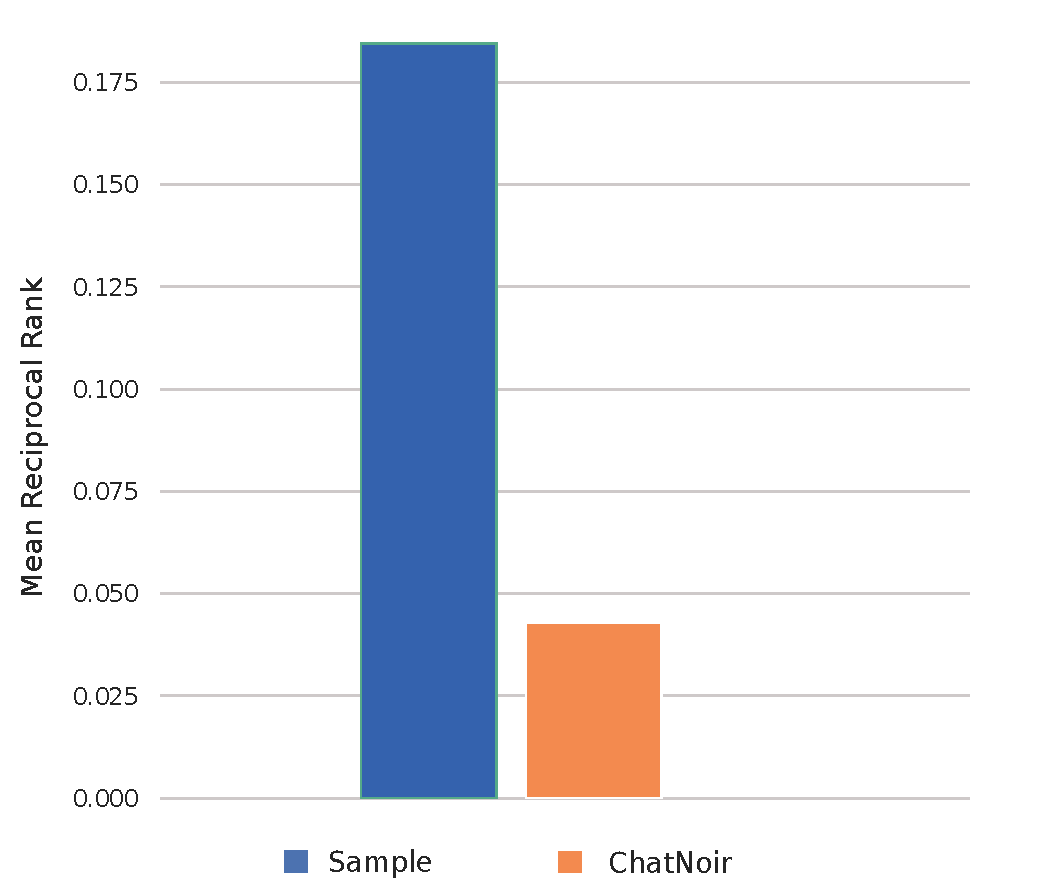
\includegraphics[width=1.0\textwidth]{graphics/evaluation/mrr_index_cw12.pdf}
    \end{minipage}
    \hfill
    \begin{minipage}[b][][b]{0.45\textwidth}
    \centering
    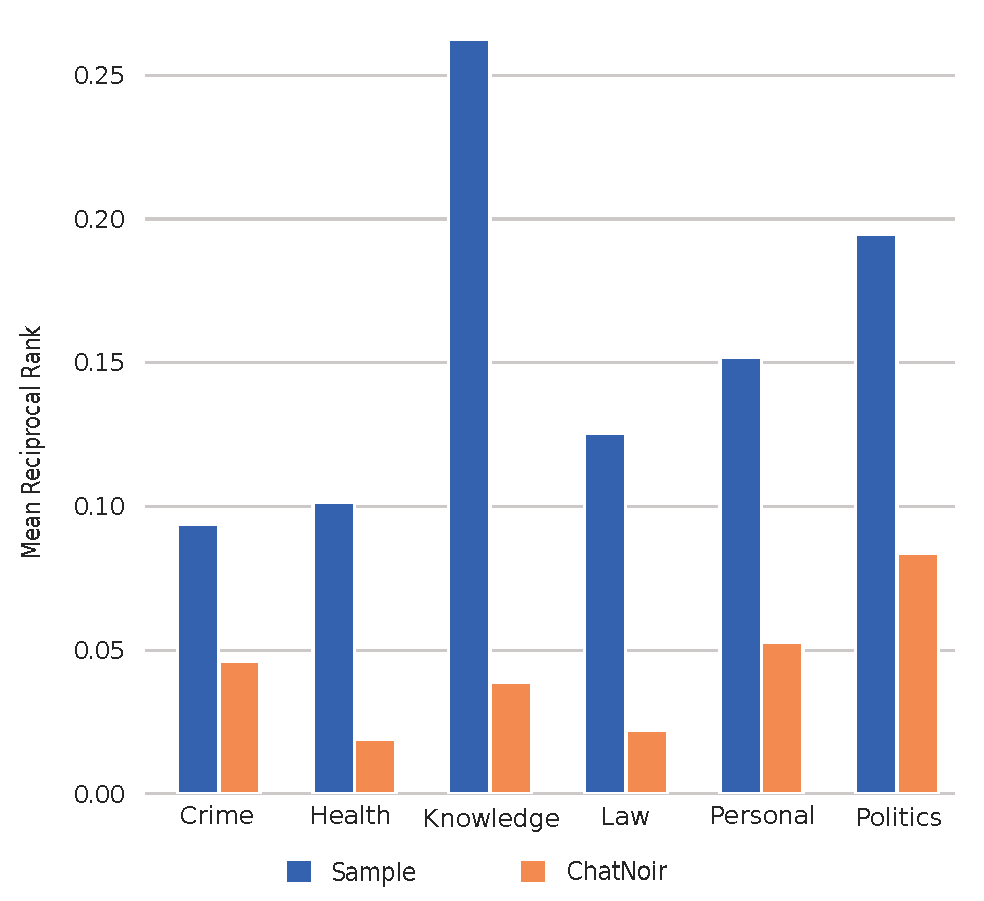
\includegraphics[width=1.0\textwidth]{graphics/evaluation/mrr_categories_both_level.pdf}
    \end{minipage}
\caption{Comparison of the Mean Reciprocal Rank for the obfuscated queries in our document sample and ChatNoir, divided into the different categories.}
    \label{fig:mrr}
\end{figure}


Through our research, we were able to identify five different query types or formulation strategies: Creative, Only Suggestions, Some Suggestions, No Suggestions, and New Word. Queries that belong to the category Creative neither contain a single word from the provided keyword list nor a word from the target document. Only Suggestions are queries that are completely made out of words from the keyword list. Queries from Some Suggestions contain at least one word from the keyword list and one additional word that is not part of the list. No Suggestions are queries that do not contain any words from the list and the last type New Word consists out of queries that have at least one term that does not come from the target document. In Figure~\ref{fig:querytypes} we can see the number of queries that belong to each query type. Note that some queries can belong to more than one type. The least used category is Creative. Although 26 players have used this strategy at least once, the proportion of queries in this category is very low. This could be due to the success rate of 0\%, which results from the BM25 ranking function. This search function needs at least one word from the target document to be able to retrieve it. We can also see this if we compare the success rate of the different categories. Figure~\ref{fig:queries:success} shows that the queries that contain at least one keyword from the list are the most successful. But the query type Only Suggestions is also not very popular. This could indicate that humans automatically try to formulate meaningful queries for them instead of simply stringing keywords together even if this would be more effective.
In the following, we will have a further look at the four query types that have a chance of retrieving the target documents.\par

\begin{table*}[t!]
    \setlength{\tabcolsep}{0.2em}
    \caption{Overview of the effectiveness of obfuscated queries in ChatNoir and the games' document sample (`Sample'). We report the Mean Reciprocal Rank (MRR), the number of documents retrieved for the original query (`Ori.'), and the number of retrieved relevant documents (`Rel.'). We show results for automatically obfuscated queries and four different types of queries submitted by players.}
    \label{table-evaluation}
    \tiny
    \begin{tabular*}{\textwidth}{@{\extracolsep{\fill}}ll@{\qquad}ccc@{\quad}cc@{\quad}cc@{\quad}cc@{\quad}cc@{}}

        \toprule

        & & & & & \multicolumn{4}{@{}c@{\quad}}{\textbf {Our Sensitive Queries}} & \multicolumn{4}{@{}c@{\quad}}{\textbf {Sensitive Web Track Queries}}\\
        
        \cmidrule(r{1em}){6-9} \cmidrule(r{.1em}){10-13}
        
        & & \multicolumn{3}{@{}c@{\quad}}{Obfuscated Queries} & \multicolumn{2}{@{}c@{\quad}}{ChatNoir} & \multicolumn{2}{@{}c@{\quad}}{Sample} & \multicolumn{2}{@{}c@{\quad}}{ChatNoir} & \multicolumn{2}{@{}c@{\quad}}{Sample}\\

        \cmidrule(r{1em}){3-5} \cmidrule(r{1em}){6-7} \cmidrule(r{1em}){8-9} \cmidrule(r{1em}){10-11} \cmidrule(r{.1em}){12-13}

        & & Count & Length & Time & MRR & Ori. & MRR & Ori. & MRR & Rel. & MRR & Rel. \\

        \midrule

        \multirow{4}{*}{\rotatebox[origin=c]{90}{\parbox[c]{4em}{\centering \textbf{Queries}}}}
        & Only Suggestions & \phantom{0}130\,/\,21\phantom{0} &  2.42 & 40.50\,s & 0.093 & 5.223 & 0.325 & 67.592 & 0.010 & 3.094 & 0.152 & 3.691\\
        
        & Some Suggestions & \phantom{0}556\,/\,125 & 4.53 & 42.45\,s & 0.046 & 4.667 & 0.258 & 85.829 & 0.013 & 3.632 & 0.038 & 3.568 \\
        
        & No Suggestions & \phantom{0}576\,/\,157 & 2.88 & 44.39\,s & 0.029 & 2.935 & 0.082 & 38.932 & 0.015 & 1.783 & 0.024 & 3.316 \\
        
        & New Word & \phantom{0}559\,/\,158 & 3.57 & 46.27\,s & 0.002 & 1.517 & 0.051 & 49.992 & 0.002 & 1.235 & 0.005 & 2.790 \\

        \midrule

        %\multirow{3}{*}{\rotatebox[origin=c]{90}{\parbox[c]{10em}{\centering \textbf{Au}}}}
        & Automatic & 1025\,/\,327 & 2.91 & --- & 0.088 & 9.229 & 0.420 & 84.264 & 0.014 & 2.872 & 0.042 & 3.743 \\
        
        \bottomrule

    \end{tabular*}
    \vspace*{-2ex}
\end{table*}

Table~\ref{table-evaluation} compares the effectiveness of the query types between each other and to queries automatically obfuscated with the approach of Arampatzis et al.~\cite{arampatzis}. Apart from the data on the different query types, the table shows an additional distinction of the queries into the sensitive queries from the Web Tracks (Sensitive Web Track Queries) and the queries from other sources in our collection (Our Sensitive Queries). For our sensitive queries, we report the Mean Reciprocal Rank (MRR) for finding the target document and the number of retrieved documents from the top-300 ranking when the original sensitive query is submitted (Ori.).
For the Web Track queries with relevance judgments, we report the MRR and the number of retrieved relevant documents (Rel.). The data indicates that the less players relied on the suggested keywords, the more time they needed to formulate their queries thus becoming less efficient (40.50 s vs. 46.27s). Overall, the time taken for the obfuscations is 40.72 seconds on average. Since we do not know how long people normally need to formulate queries, we cannot say anything about whether this is within the normal range or make any kind of comparison. But since there exist some cases in which the needed time exceeds this average value by far, there must have been some players that took their time to thoroughly inspect the provided information.\par
As expected and as we have seen before, the MRR for the index is always better than for ChatNoir which is caused by the difference in the number of documents.
Based on our collected data we can conclude that the further players deviates from the provided keywords, the less effective their query will be. This is equally true for the target web page, the number of related or relevant documents as well as the time taken to formulate an obfuscated query. If we compare the obfuscated queries of humans with automatically generated queries, then we see that players who use only terms from or list of keywords (Only Suggestions) slightly improve upon automatic obfuscation (MRR of 0.093 vs. 0.088). But for all other query types, this does not hold. On the contrary, the MRR for the automatic queries exceeds the MRR for the human-made queries. This is especially the case for the category New Word for which the obfuscations are rather useless (MRR of 0.002). With an MRR this low, no real search engine user would look at the target document, since most of them are not even interested in documents positioned worse than the tenth result~\cite{pictureSearch}. The findings of this paragraph are also confirmed by the data of the sensitive Web Track queries.
\begin{figure}[ht!]
    \vspace*{-.4cm}
    \begin{minipage}[b][][b]{0.45\textwidth}
    %\centering
    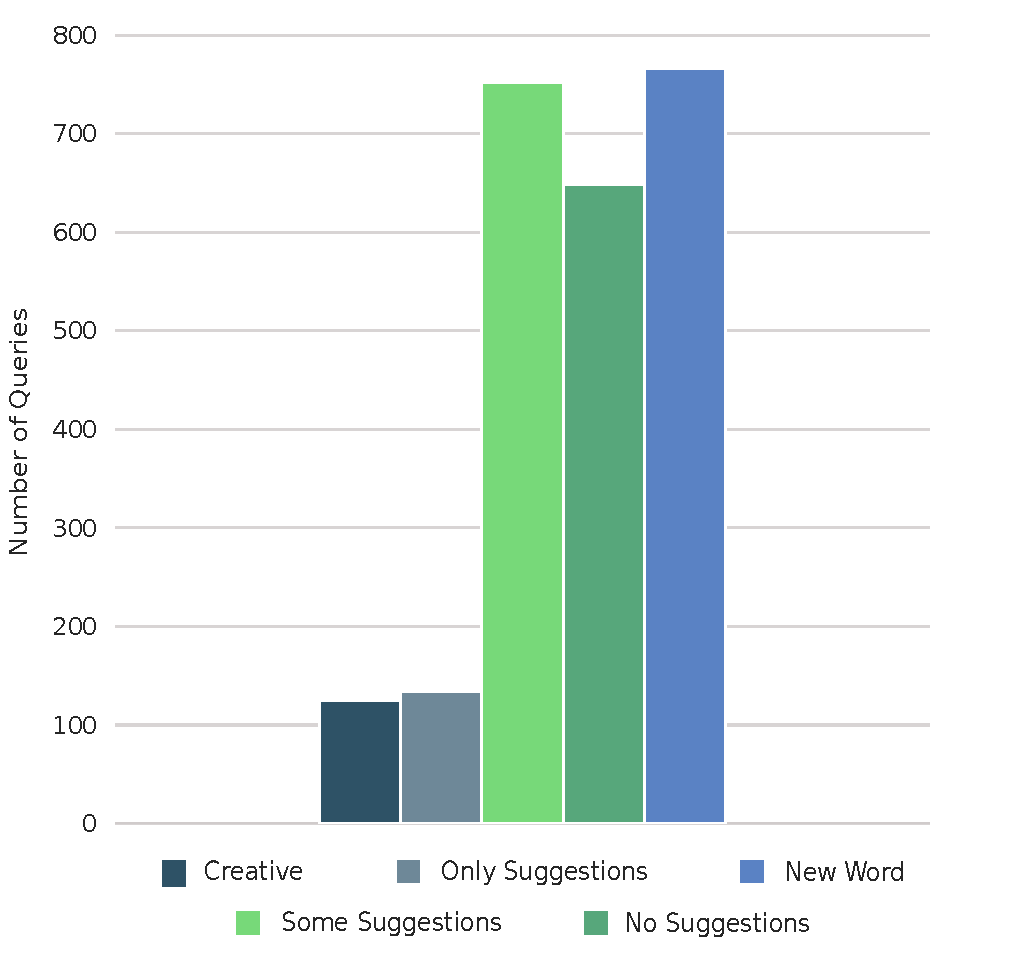
\includegraphics[width=1.0\textwidth]{graphics/evaluation/five_query_categories.pdf}
    \caption{Overview of the number of queries in each query type.}
    \label{fig:querytypes}
    \end{minipage}
    \hfill
    \begin{minipage}[b][][b]{0.45\textwidth}
    %\centering
    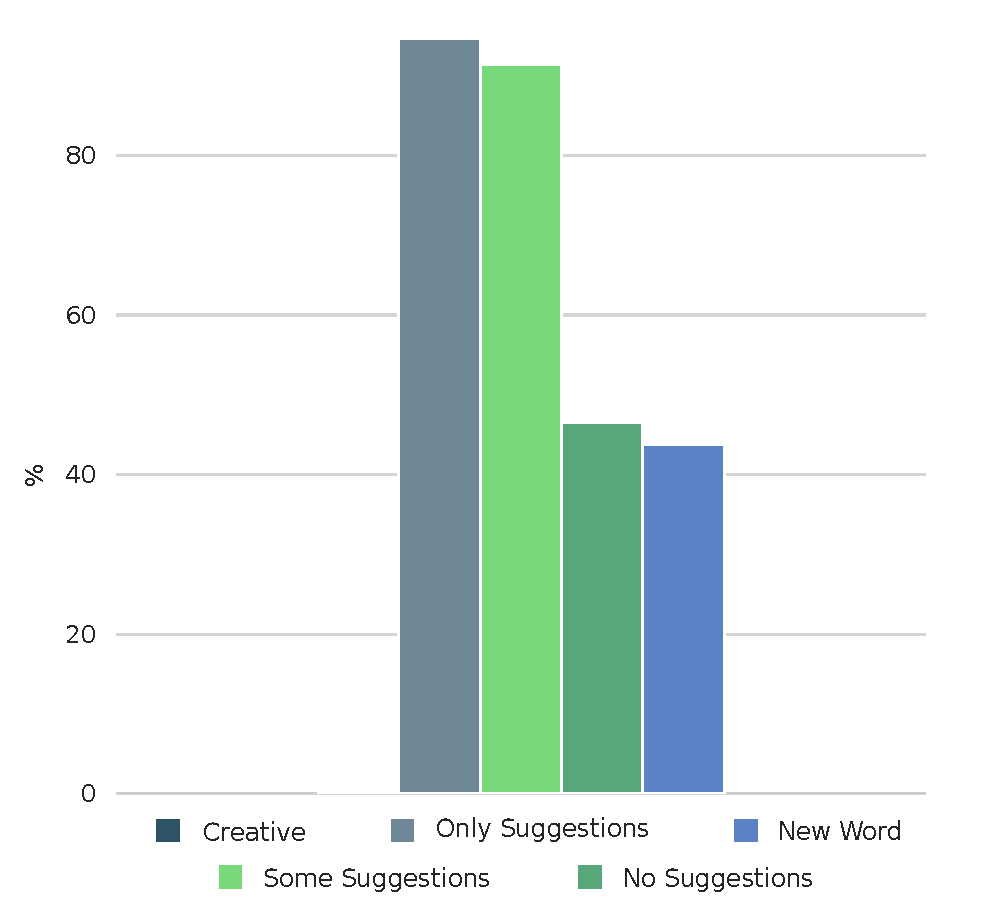
\includegraphics[width=1.0\textwidth]{graphics/evaluation/five_query_categories_success_rate.pdf}
    \caption{Overview of the success rate of players for each query type.}
    \label{fig:queries:success}
    \end{minipage}
\end{figure}


